\documentclass[spanish, fleqn]{article}
\usepackage[utf8]{inputenc}
\usepackage{graphicx}
\usepackage{amsmath}
\usepackage{bm}
\usepackage{tikz}
\usepackage{adjustbox}
\usepackage[top=3cm,bottom=3cm,left=3.5cm,right=3.5cm,footskip=1.5cm,headheight=1.5cm,headsep=.5cm,textheight=3cm]{geometry}

\begin{document}
\title{Inteligencia Artificial \\ \begin{Large}Estado del Arte: The Progressive Party Problem\end{Large}}
\author{Pablo Ibarra S.}
\date{\today}
\maketitle

\section*{Evaluación}

\begin{tabular}{ll}
Resumen (5\%): & \underline{\hspace{2cm}} \\
Introducción (5\%):  & \underline{\hspace{2cm}} \\
Definición del Problema (10\%):  & \underline{\hspace{2cm}} \\
Estado del Arte (35\%):  & \underline{\hspace{2cm}} \\
Modelo Matemático (20\%): &  \underline{\hspace{2cm}}\\
Conclusiones (20\%): &  \underline{\hspace{2cm}}\\
Bibliografía (5\%): & \underline{\hspace{2cm}}\\
 &  \\
\textbf{Nota Final (100\%)}:   & \underline{\hspace{2cm}}
\end{tabular}

\begin{abstract}
En este informe se presenta un estado del arte del problema conocido como \textit{Progressive Party Problem}. El problema consiste en programar de la mejor manera una fiesta de yates, donde distintas personas visitaran varios yates anfitriones. Además, se definen términos y conceptos importantes utilizados en la literatura e investigaciones en el área. Se explica y define el problema a tratar, así como también se realizan descripciones y clasificaciones de las distintas variantes que se han desarrollado a través de los años. Se describen las distintas estrategias y algoritmos que se han desarrollado para la resolución del problema principal junto a sus variantes y se presentan también modelos matemáticos del problema.

\end{abstract}

\section{Introducción}

Hoy en día la programación de horarios es un tema vital para personas y organizaciones, debido a que si se realiza bien, los recursos que se disponen y utilizan, se distribuirán de manera eficiente e inteligente. La programación lineal entera a sido una herramienta clave durante mucho tiempo para resolver este tipo de problemas, aun así, existen ciertos problemas que PLE no puede resolver debido a la explosión combinatorial de estos problemas, un ejemplo de un problema que presenta estas características es el problema llamado \textit{Progressive Party Problem} y será nuestro foco de estudio en el presente informe.

El problema conocido como Progressive Party Problem fue introducido por Peter Hubbard miembro de la asociación de propietarios SeaWych y del departamento de matemáticas de la universidad de Southampton, cuando tuvo que organizar una fiesta de yates en la isla Wight el años 1996, que se encuentra al sur de la costa de Inglaterra. El problema nos sitúa en el contexto de una fiesta de yates durante la tarde, donde la tripulación de cada yate debe interactuar socialmente con las otras tripulaciones. 

El propósito de este informe es investigar sobre dicho problema, sobre los métodos que existen para solucionarlo, presentar antecedentes de lo que se a desarrollado, presentar hacia donde apuntan las nuevas investigaciones y presentar un modelo matemático del problema.

La motivación de este problema es debido a la importancia que tiene en problemas reales. Inicialmente se planteó como un problema para la organización de fiesta en yates, pero hoy en día su estudio puede ayudar para organizar de mejor manera ferias de libros, tours y otro tipo de eventos, optimizando los recursos de estos con el fin de maximizar el beneficio, por ejemplo, ganancias.

En este informe se presenta información relevante para poder introducirse al tema de \textit{Progressive Party Problem}. Primero se comienza definiendo el problema a estudiar y se presentan otras variantes conocidas que existen del problema. Luego le sigue una sección centrada en el Estado del Arte del problema, donde se explican los métodos mas importantes que existen de resolución para este tipo de problema. Para aportar al estudio del problema este informe presenta, en otra sección, distintos modelos matemáticos que pueden ser usados para poder solucionar el problema mediante técnicas de optimización. Finalmente, el informe concluye con unas conclusiones respecto al tema y lo que puede venir en el futuro respecto a este.


\section{Definición del problema}

El problema \textit{Progresive Party Problem} descrito por Peter Hubbard habla de un total de 39 botes que participan en la fiesta, algunos de estos son seleccionados para ser yates anfitriones, la tripulación de los yates anfitriones deben mantenerse en su bote ya que tienen que organizar la fiesta en sus barcos, mientras que las otras tripulaciones, que son conocidos como tripulación huésped, se pasean por los yates anfitriones socializando con el resto de las tripulaciones. La fiesta completa dura 3 horas, por lo que las tripulaciones huéspedes deben ir rotando cada 30 minutos para que socialicen lo que mas puedan. La tripulación de cada barco se mantiene junta y cada barco tiene una capacidad máxima. Por otro lado el barco del organizador de la fiesta siempre debe ser anfitrión, independiente de la capacidad del bote, esto es por que en ese barco estarán todos los elementos para enfrentar una eventual emergencia. Debido a que el organizador y dos tripulaciones mas (Estas tripulaciones deberán ser anfitriones y corresponden ser las tripulaciones del bote 1,2 y 3) tienen niños entre sus tripulaciones  se crearon tres botes virtuales con capacidad 0, uno por cada anfitrión, esto se hizo debido a que solo los adultos son anfitriones de los yates designados como anfitriones, por lo tanto el problema final se consideran 42 botes. Finalmente lo que se busca en este problema es minimizar la cantidad de barcos anfitriones (debido a que se tienen que abastecer con comida) y asignar las tripulaciones huéspedes a cada yate anfitrión durante todos los intervalos de tiempo que dure la fiesta. La Data para el problema dado esta en la siguiente tabla.


\begin{figure}[!h]
  \centering
    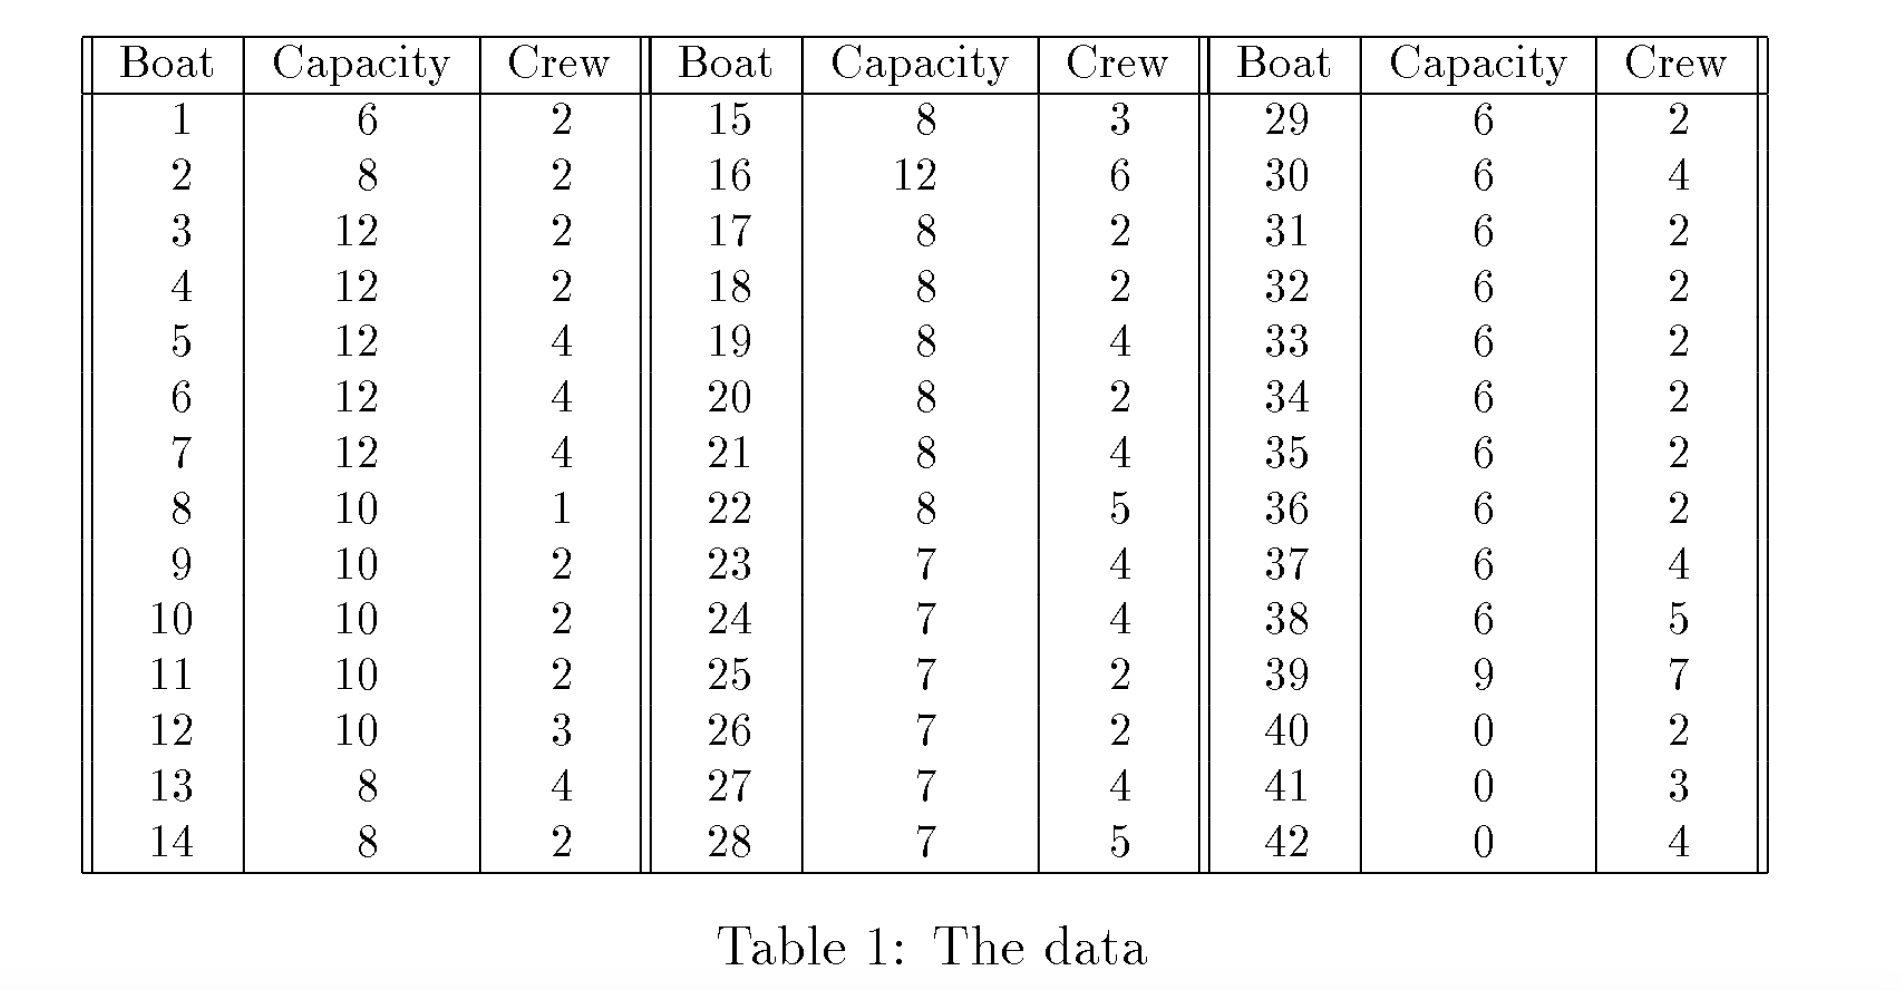
\includegraphics[width=0.7\textwidth]{1}
  \label{fig:DiagramaBarra2}
\end{figure}

\newpage

Por lo tanto identificamos 42 botes (tripulaciones), definimos $\mathit{i},\mathit{j},\mathit{k} \in \{1,..,42\}$ y un conjunto de tiempos $\mathit{t} \in \{1,...,6\}$.

\begin{enumerate}
\item El tamaño de las tripulaciones estará dada por $\mathit{s}_{\mathit{i}}$, y la capacidad del bote - la máxima cantidad de personas que el bote puede recibir incluyendo los dueños del bote es de $\mathit{C}_{\mathit{i}}$.

\item El número máximo de invitados que puede cada bote invitar es de $\mathit{c}_{\mathit{i}}$ = max (0,$\mathit{C}_{\mathit{i}}$-$\mathit{s}_{\mathit{i}}$).

\item Se introduce la variable binaria $\mathit{x}_{\mathit{i},\mathit{j},\mathit{t}}$. La variable $\mathit{x}_{\mathit{i},\mathit{j},\mathit{t}}$ = 1 si la tripulación huésped $\mathit{j}$ visita a la tripulación anfitriona $\mathit{i}$ en el periodo de tiempo $\mathit{t}$. En todo otro caso $\mathit{x}_{\mathit{i},\mathit{j},\mathit{t}}$ = 0.

\item Se utiliza otra variable binaria para decidir cuales botes son anfitriones. La variable $\mathit{h}_{\mathit{i}}$ = 1 si el bote $\mathit{i}$ es anfitrión, en el caso que el bote sea huésped $\mathit{h}_{\mathit{i}}$ = 0.

\item Solo hay fiestas en los botes anfitriones, o, si una tripulación huésped visita a un bote $\mathit{i}$ en algún periodo de tiempo, entonces el bote $\mathit{i}$ es anfitrión.

\item La capacidad máxima de cada bote nunca se puede exceder.

\item No hay tripulaciones hibridas, esto quiere decir que una tripulación es anfitrión o es huésped.

\item Una tripulación $\mathit{j}$ visita a otra tripulación $\mathit{i}$ al menos una vez.

\item Los botes 1,2 y 3 tienen que ser anfitriones. (Barco del organizador y 2 barcos que tenían tripulación con niños).

\item Los botes 40,41 y 42 deben ser botes huéspedes con capacidad 0 (Barco virtual de niños).

\item Las tripulaciones huéspedes no pueden encontrarse más de una vez durante toda la fiesta, esta restricción genera una nueva variable $\mathit{m}_{\mathit{j},\mathit{k},\mathit{t}}$ donde toma valor 1 si una tripulación $\mathit{j}$ y una tripulación $\mathit{k}$ se encuentran en una fiesta en el periodo $\mathit{t}$.

\item Finalmente lo que se busca es minimizar el número de barcos anfitriones, seleccionar que barcos serán los anfitriones y asignar las tripulaciones huéspedes a los barcos anfitriones durante todo lo que dure la fiesta.

\end{enumerate}

El problema en su estructura a permanecido igual durante todos estos años, las variaciones que se proponen son simplemente relajaciones del problema original.


\subsubsection*{The Uncapacitated Problem~\cite{Smith1996}}

La primera variante que se intentó resolver de \textit{Progressive Party Problem} fue resolver el problema sin considerar la capacidad de los barcos, esto quiere decir que un barco puede almacenar a todas las tripulaciones huéspedes en un solo periodo. Ahora si pensamos en más de un periodo, es fácil ver una cota inferior de barcos anfitriones que necesitaremos para la fiesta, si $\mathit{g}$ tripulaciones huéspedes visitan el barco anfitrión $\mathit{i}$ en el periodo 1, necesitaremos al menos $\mathit{g}$ barcos anfitriones en el periodo 2 (Esto es debido a que no podemos volver a visitar el barco $\mathit{i}$ y además las tripulaciones huéspedes no pueden volver a encontrarse). Por lo tanto, necesitaremos $\mathit{g}$ +1 barcos anfitriones para que las tripulaciones del periodo 1 no se encuentren en el periodo 2, entonces claramente $\mathit{g}$($\mathit{g}$+1) es la cantidad máxima de tripulación huésped que podemos acomodar en los 2 periodos utilizando solo g+1 barcos anfitriones. Usando lo anterior, para una instancia de 6 anfitriones podemos acomodar 30 huéspedes, para una instancia de 7 anfitriones podemos acomodar 42 huéspedes. Para el caso en particular de 42 botes en total, 7 serán anfitriones (35 huéspedes). Ahora como en la vida real los barcos tienen una capacidad máxima, por lo tanto, este enfoque no es el más indicado.

 
 \newpage
 
\subsubsection*{A Lower Bound~\cite{Smith1996}}

Considerar la capacidad de los barcos es muy importante si es que se quiere encontrar una solución aceptable para este problema, es por esto que se buscó otro enfoque. La segunda variante propuesta del problema, también una relajación, es resolver el problema considerando que no existen distintas tripulaciones huéspedes, si no que existe una única y gigante tripulación huésped. Lo que se busca con esto es encontrar cual es la cantidad de botes anfitriones que se necesitan para que quepan toda la tripulación huésped en el primer periodo. Lo que no se esta considerando acá es que los miembros de cada tripulación deban permanecer juntos.

\subsubsection*{Otras Variantes~\cite{Smith1996}}

Otra variante del problema es resolver el problema como un CSP, es decir, encontrar una instanciación de las variables que cumpla las restricciones sin una función objetivo. Finalmente, la última variante que nombraremos será cambiar la función objetivo de tal manera de maximizar la cantidad de periodos, con el fin de que la fiesta dure más.


\section*{Estado del Arte}

Como el problema data del año 1996, muchos autores han propuesto estrategias y algoritmos para resolver el Progressive Party Problem, algunos de estos metodos utilizados los presentaremos en esta sección

\begin{itemize}
\item Los primeros métodos~\cite{Smith1996} se comenzaron a proponer en 1996, el mismo autor del problema, Peter Hubbard y su equipo comenzaron a resolver dos variantes del problema del \textit{Progressive Party Problem}, estas fueron las variantes \textit{The Uncapacitated Problem} y \textit{Lower Bound}. El fin de resolver estos dos problemas fue para encontrar una cota inferior sobre la cantidad de botes anfitriones que se necesitarían para cierta cantidad de tripulaciones huéspedes.
Luego de haber resuelto los dos problemas anteriores, Peter y su equipo hicieron dos formulaciones usando programación lineal entera con el fin de resolver el problema. 

La primera formulación se utilizaron variables binarias para resolver un CSOP con el objetivo de minimizar la cantidad de barcos anfitriones, el número de restricciones de este modelamiento fue del orden de O($B^{4}T^{2}$), donde B es el número de botes y T la cantidad de periodos, el numero variables fue moderado, alrededor de O($B^{2}T$). Se corrieron pruebas utilizando 14 botes y 4 periodos de tiempo, el modelo resulto tener 379 variables y 18212 filas, el resultado fue obtenido después de 259 segundos utilizando XPRESSMO optimiser[ref] en una IBM 486 DX PC, en tan solo 816 iteraciones.

La segunda formulación también se utilizó variables binarias, se hicieron algunos cambios en las restricciones, el objetivo de esta formulación fue el reducir la cantidad de restricciones, lográndose bajar a O($B^{3}T$) pero con el costo de que aumentaron el número de variables a O($B^{3}T$). Las mismas pruebas que se realizaron en la primera formulación se utilizaron con este segundo modelo, obteniendo los mismos resultados, pero en un tiempo menor.

Finalmente, cuando se intentó resolver el problema completo utilizando las dos formulaciones anteriores, se falló con ambas modelos. Debido a lo anterior se decidió relajar el problema, fijando que el mínimo número de barcos anfitriones deberían estar entre 13 y 15 (Esto se basó en los resultados obtenidos de las cotas inferiores obtenidas en los problemas \textit{the Uncapacitated Proble}m y \textit{Lower Bound}), además se ignoró la restricción de que las tripulaciones huéspedes se puedan encontrar mas de una vez, la solución fue encontrada en 598 segundos. Al ver que esta heurística funcionaba, la de fijar un rango en la cantidad de botes anfitriones, se corrió un segundo intento, que fallo al no arrojar ningún resultado luego de 189 horas.

Luego de que los modelos de programación lineal fallaran, el equipo modelo el \textit{Progressive Party Problem} como un CSP, se logra eliminar la función objetivo ya que previamente se definen quienes serán los 13 barcos anfitriones, se eligen 13 debido a la cota inferior que se encontró previamente cuando se pensó en una gran tripulación huésped. Este CSP fue resuelto usando una librería de C++ llamada ILOG Solver, la librería posee una implementación de backtracking con full lookahead. La ventaja que tiene este modelo de estilo CSP es la cantidad de variables y restricciones que estas tienen, ambas están alrededor de O($B^{2}T$). Finalmente se logró encontrar una resultado utilizando 13 botes anfitriones, 29 huéspedes y 6 periodos en 27 minutos, también arrojo buenos resultados con 7 y 8 periodos.


\begin{figure}[!h]
  \centering
    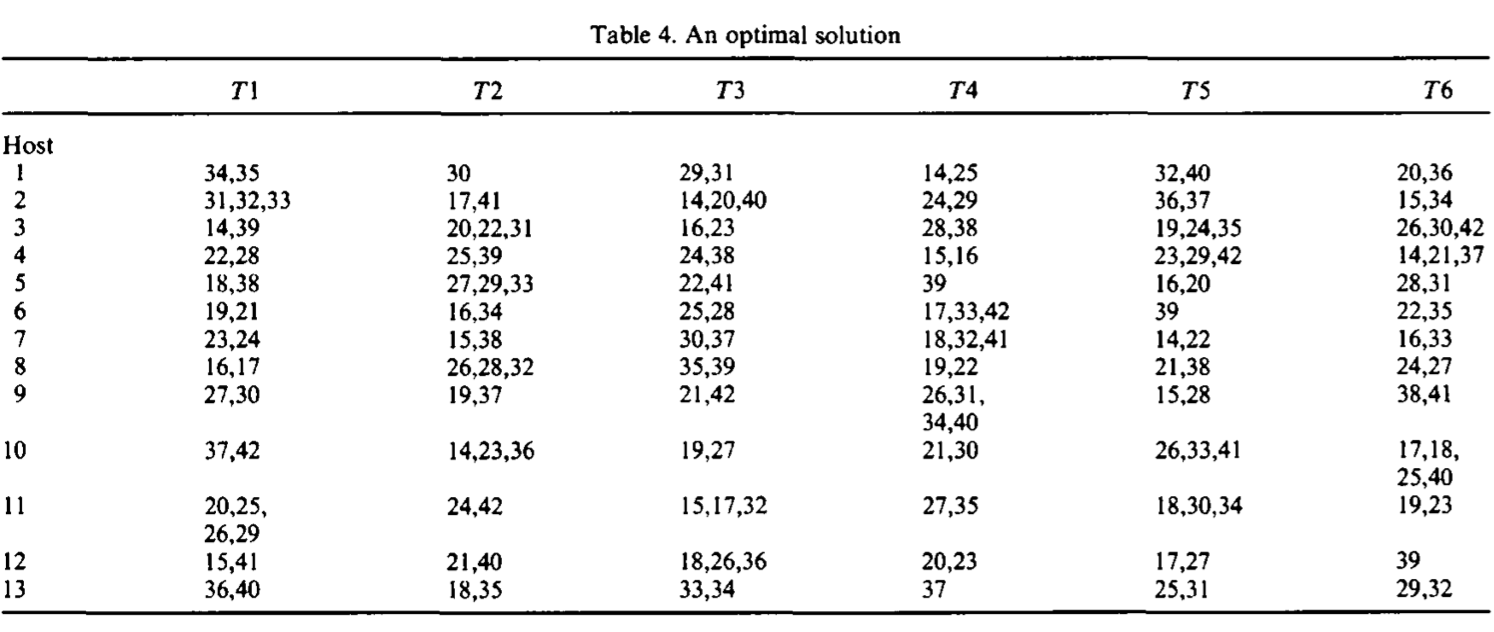
\includegraphics[width=0.9\textwidth]{2}
    \caption{Ejemplo de solución optima}
  \label{fig:DiagramaBarra3}
\end{figure}


\item En 1997, Joachim P. Walser~\cite{Walser:1997:SLP:1867406.1867448} fue uno de los pioneros en utilizar algoritmos de búsqueda local para resolver este problema, el algoritmo que lleva por nombre WSAT, realiza una búsqueda local usando Greedy con restricciones pseudo-booleanas, además viene con un mecanismo de historial y una lista tabú. Este algoritmo trabaja dentro del mundo de lo factible, se define un movimiento, y cada vez que se realiza este se va calculando un score, si este score disminuye nos vamos quedando con la nueva instanciación, cuando el score llega a 0 quiere decir que estamos en presencia de la solución óptima.  En caso de que exista un empate entre score, se utiliza la lista historia para regresar a la instanciación mas antigua, obviamente ignorando las instanciaciones que se encuentran en la lista tabú. Para resolver el \textit{Progressive Party Problem}, Walser se baso en el trabajo hecho por Peter Hubbard y su equipo, utilizo el mismo modelo CSP, utilizo los 13 botes propuestos por Peter Hubbard y además genero 5 instanciaciones de los 13 botes iniciales considerados como anfitriones(Asegurándose que la capacidad de los 13 botes sean suficiente para las tripulación huésped), además se modificaron ciertas restricciones del CSP original a restricciones del tipo Pseudo-Boleanas y finalmente, se fijó el tamaño de la lista tabú en 1. Se obtuvieron los siguientes resultados.

\newpage 

\begin{figure}[!h]
  \centering
    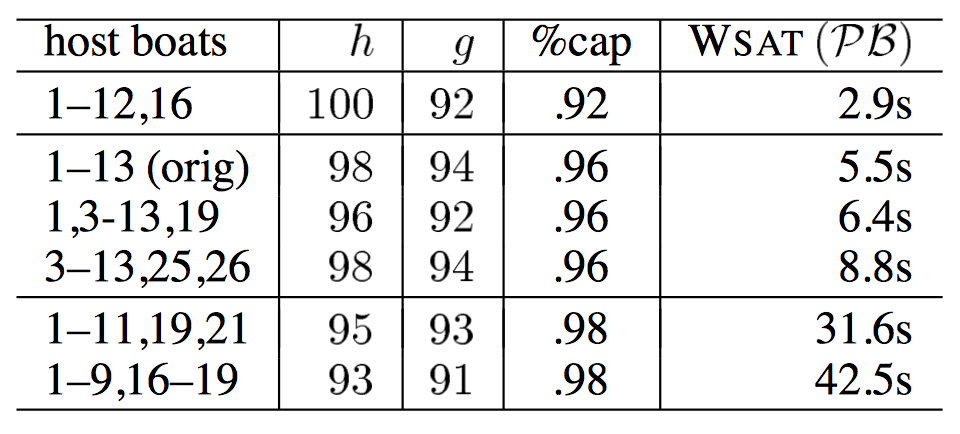
\includegraphics[width=0.4\textwidth]{3}
  \label{fig:DiagramaBarra4}
\end{figure}

La tabla anterior muestra los botes anfitriones seleccionados, la capacidad máxima de los botes, la cantidad total de huéspedes, porcentaje total de la capacidad utilizada y tiempo promedio de correr el algoritmo 20 veces, los resultados fueron considerablemente más bajo que el modelo propuesto por el trabajo de Peter Hubbard. Adicionalmente se resolvió el CSP original utilizando Oz, un lenguaje de restricción concurrente, con el fin de comparar con el Solver ILOG que se utilizó inicialmente para resolver el problema, el tiempo que demoro Oz fue de 8 minutos, en una maquina conocida como SPARCstation 20, en cambio, el Solver ILOG demoro 27 minutos, también se aprecia una disminución notable en el tiempo de resolución del problema.

\item En 1999 Philippe Galinier junto a Jin-Kao Hao propusieron una tercera forma~\cite{Galinier1999}  de resolver este problema, su método de resolución se basa en búsqueda local, trabajando en el mundo de lo infactible resolviendo el CSP propuesto por Peter Hubbard y su equipo. Para resolver el \textit{Progressive Party Problem}, ellos introducen un espacio de búsqueda, una función de costo y dos diferentes vecindarios, donde se experimentan con ambos utilizando distintas heurísticas. El espacio de búsqueda que ellos utilizan es de G x T, donde G es igual a 29 y T $\in$ (6,7,8,9,10), este espacio de búsqueda se justifica dado que el CSP ya están asignados los 13 barcos anfitriones, por lo tanto, debemos asignar las 29 tripulaciones en los t periodos que definamos. La función de costo que proponen es una función que castiga cada restricción incumplida, castigando más a las restricciones duras que las blandas. Los dos vecindarios que generan dependen de los dos movimientos que ellos proponen, el primer movimiento corresponde a cambiar el barco anfitrión de una tripulación huésped con conflicto, esto quiere decir que se irán probando distintos barcos anfitriones quedándose con el barco anfitrión que presente menos conflictos. El segundo movimiento corresponde a hacer un \textit{swap} entre los barcos anfitriones asignados a dos tripulaciones huéspedes. Ya definido lo anterior, Galinier y Hao utilizan dos algoritmos para resolver el problema, uno de ellos es \textit{taboo search}~\cite{Glover:1997:TS:549765} y el segundo es conocido como metrópolis (Versión simplificada de \textit{Simulated Annealing}~\cite{Kirkpatrick671}. Finalmente, se definen cuatro criterios de parada


\begin{enumerate}
	\item Si la función de costo es igual a 0.
	\item Si se alcanza el tiempo máximo establecido para que el algoritmo se ejecute.
	\item Si se alcanza el máximo numero de iteraciones.
	\item Si se alcanza el máximo numero de movimientos.

\end{enumerate}

La implementación fue realizada en C++ y ejecutada en una maquina conocida como Sun ULTRA 1. Los resultados se muestra en una tabla donde se compara el tiempo que demora en encontrar una solución utilizando ILP(\textit{Integer Linear Programing}) y la resolución del CSP propuestos por Peter Hubbard vs los algoritmos de búsqueda local propuestos.


\newpage


\begin{table}[h!]
\centering
   \begin{tabular}{|l|l|l|l|}
    \hline
    Problem & ILP  & Publisher CSP resolution & LS     \\ \hline
    p6      & fail & 27 min                   & $<$ 1 s. \\
    p7      & fail & 28 min                   & $<$1 s. \\
    p8      & fail & fail                     & 1 s.   \\
    p9      & fail & fail                     & 4 s.   \\
    p10     & fail & fail                     & fail   \\ \hline
    \end{tabular}
\end{table}

Se corrieron los experimentos 20 veces, el tiempo promedio obtenido por los algoritmos de búsqueda local son muchos más bajos que los resueltos por ILOG Solver. Si bien los algoritmos pudieron resolver para 6,7,8 y 9 periodos, observamos que para 10 periodos el algoritmo falla en resolver el problema. Para finalizar observemos la siguiente tabla del costo entregado al intentar resolver el problema con 9 periodos de tiempo utilizando los algoritmos de  búsqueda local.


\begin{figure}[!h]
  \centering
    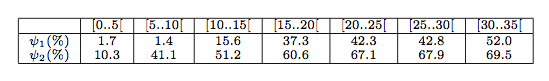
\includegraphics[width=0.8\textwidth]{4}
  \label{fig:DiagramaBarra5}
\end{figure}

La tabla indica en cada columna el porcentaje de soluciones que tuvieron un costo dentro de ese intervalo a medida que el algoritmo fue iterando, es decir, en la primera columna nos dice que el 1.7$\%$ de los resultados obtenidos redujeron su costo a 0,1,2,3 o 4. Esta información es importante ya que nos permite comparar y observar que el segundo movimiento tiende a mejorar mucho más la solución que el primer movimiento. Es importante también notar que estos métodos encuentran óptimos globales como óptimos locales.

\item En el año 2001, Erwin Kalvelagen, propuso un modelo~\cite{Kalvelagen20031713} basado en programación lineal mixta, este enfoque logro que la programación lineal pudiese resolver el problema de manera completa utilizando 7 periodos. El modelo se testeo en un software llamado GAMS(textit{Software} especializado en resolver modelos matemáticos) sobre una maquina Cray C90. El modelo generado tuvo las siguientes características.


\begin{figure}[!h]
  \centering
    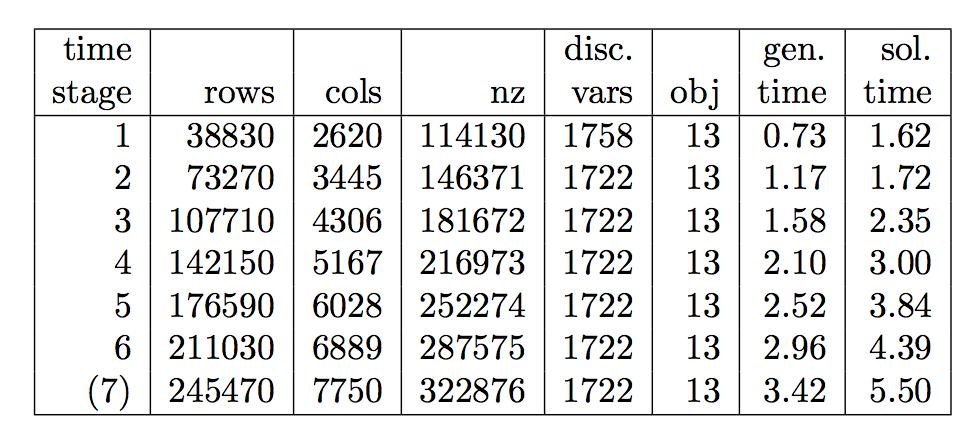
\includegraphics[width=0.6\textwidth]{5}
  \label{fig:DiagramaBarra5}
\end{figure}

En la tabla anterior las filas corresponden ser a la cantidad de restricciones que tenemos, las columnas son la cantidad de variables, nz la cantidad de elementos que no son ceros, disc. vars corresponde a la cantidad de variables discretas, obj corresponde al optimo encontrado por la función objetivo, gen. time el tiempo que demora en generar el modelo y sol. time el tiempo que demora en encontrar una solución para el periodo t. Podemos observar de la tabla que la cantidad de variables y restricciones va aumentando a medida que pasan los periodos, en consecuencia, el tiempo que demora en encontrar una solución también va en aumento.


\end{itemize}

\newpage

\section{Modelo Matematico}

En esta sección se nombraran los dos modelos mas importantes que tuvieron un gran protagonismo en el estado del arte

\subsection*{Modelo CSOP~\cite{Kalvelagen20031713}~\cite{Smith1996}}
El modelo matemático que se muestra a continuación es el CSOP propuesto por Peter Hubbard. Se identifican 42 botes (tripulaciones), definimos $\mathit{i},\mathit{j},\mathit{k} \in \{1,..,42\}$ y un conjunto de tiempos $\mathit{t} \in \{1,...,6\}$.
\begin{enumerate}
\item El tamaño de las tripulaciones estará dada por $\mathit{s}_{\mathit{i}}$, y la capacidad del bote - la máxima cantidad de personas que el bote puede recibir incluyendo los dueños del bote es de $\mathit{C}_{\mathit{i}}$.

\item El número máximo de invitados que puede cada bote invitar es de $\mathit{c}_{\mathit{i}}$ = max (0,$\mathit{C}_{\mathit{i}}$-$\mathit{s}_{\mathit{i}}$).

\item Se introduce la variable binaria $\mathit{x}_{\mathit{i},\mathit{j},\mathit{t}}$. La variable $\mathit{x}_{\mathit{i},\mathit{j},\mathit{t}}$ = 1 si la tripulación huésped $\mathit{j}$ visita a la tripulación anfitriona $\mathit{i}$ en el periodo de tiempo $\mathit{t}$. En todo otro caso $\mathit{x}_{\mathit{i},\mathit{j},\mathit{t}}$ = 0.

\item Se utiliza otra variable binaria para decidir cuales botes son anfitriones. La variable $\mathit{h}_{\mathit{i}}$ = 1 si el bote $\mathit{i}$ es anfitrion, en el caso que el bote sea huésped $\mathit{h}_{\mathit{i}}$ = 0.

\item Solo hay fiestas en los botes anfitriones, o, si una tripulación huésped visita a un bote $\mathit{i}$ en algún periodo de tiempo, entonces el bote $\mathit{i}$ es anfitrión.

\begin{center}
$\mathit{x}_{\mathit{i},\mathit{j},\mathit{t}}$ $\rightarrow$ $\mathit{h}_{\mathit{i}}$ ($\mathit{x}_{\mathit{i},\mathit{j},\mathit{t}} \leq $  $\mathit{h}_{\mathit{i}}$) para todo $\mathit{i},\mathit{j},\mathit{t}$ ($\mathit{i} \neq \mathit{j}$)
\end{center}

\item La capacidad máxima de cada bote nunca se puede exceder.

\begin{center}
$\displaystyle \sum_{\mathit{j} \mid \mathit{i} \neq \mathit{j}}$ $ \mathit{s}_{\mathit{j}} \mathit{x}_{\mathit{i},\mathit{j},\mathit{t}} \leq \mathit{c}_{\mathit{i}} \mathit{h}_{\mathit{i}}$ para todo $ \mathit{i},\mathit{t}$
\end{center}

\item No hay tripulaciones hibridas, esto quiere decir que una tripulación es anfitrión o es huésped.

\begin{center}
$\mathit{h}_{\mathit{j}}$ + $ \displaystyle \sum_{\mathit{i}} \mathit{x}_{\mathit{i},\mathit{j},\mathit{t}}$ = 1 para todo $ \mathit{j},\mathit{t}$
\end{center}

\item Una tripulación $\mathit{j}$ visita a otra tripulación $\mathit{i}$ al menos una vez.

\begin{center}
$ \displaystyle \sum_{\mathit{t}} \mathit{x}_{\mathit{i},\mathit{j},\mathit{t}} \leq \mathit{h}_{\mathit{i}}$ para todo $\mathit{i},\mathit{j}$ ($\mathit{i} \neq \mathit{j}$)
\end{center}

\item Los botes 1,2 y 3 tienen que ser anfitriones. (Barco del organizador y 2 barcos que tenían tripulación con niños).

\begin{center}
$  \mathit{h}_{\mathit{i}}$ = 1 para todo $ \mathit{i} =$ $\{1,2,3\}$
\end{center}

\item Los botes 40,41 y 42 deben ser botes huéspedes con capacidad 0 (Barco virtual de niños).

\begin{center}
$  \mathit{h}_{\mathit{i}}$ = 0 para todo $ \mathit{i} =$ $\{40,41,42\}$
\end{center}

\item Las tripulaciones huéspedes no pueden encontrarse mas de una vez durante toda la fiesta.

\begin{center}
$\displaystyle \sum_{\mathit{j} \mid \mathit{i} \neq \mathit{j},\mathit{i} \neq \mathit{k}}$ ($\mathit{x}_{\mathit{i},\mathit{j},\mathit{t}} \wedge \mathit{x}_{\mathit{i},\mathit{j},\mathit{t}}$)$\leq $ 1 para todo $ \mathit{j},\mathit{k}$ ($\mathit{j} \neq \mathit{k}$)
\end{center}

Desafortunadamente esta restricción es difícil de resolver. Por lo tanto se introduce una nueva variable $\mathit{m}_{\mathit{j},\mathit{k},\mathit{t}}$ donde toma valor 1 si una tripulación $\mathit{j}$ y una tripulación $\mathit{k}$ se encuentran en una fiesta en el periodo $\mathit{t}$. Por lo tanto, la restricción anterior se cambia por:

\begin{center}
$\mathit{m}_{\mathit{j},\mathit{k},\mathit{t}}$ $\geq$ $\mathit{x}_{\mathit{i},\mathit{j},\mathit{t}} + \mathit{x}_{\mathit{i},\mathit{k},\mathit{t}}$ - 1 para todo  $\mathit{i},\mathit{j},\mathit{k},\mathit{t}$, ($\mathit{j} < \mathit{k}, \mathit{i} \neq \mathit{j}, \mathit{i} \neq \mathit{k}$)

$ \displaystyle \sum_{\mathit{t}} \mathit{m}_{\mathit{j},\mathit{k},\mathit{t}} \leq $1 para todo $\mathit{j},\mathit{k}$, ($\mathit{j} < \mathit{k}$)
\end{center}

La inecuación es interpretada como: Si la tripulación $\mathit{j}$ y $\mathit{k}$ se conocen en el barco $\mathit{i}$ en $\mathit{t}$ entonces es claro que  $\mathit{x}_{\mathit{i},\mathit{j},\mathit{t}}$ y  $\mathit{x}_{\mathit{i},\mathit{k},\mathit{t}}$ ambos son verdaderas, entonces $\mathit{m}_{\mathit{j},\mathit{k},\mathit{t}}$ $\geq$ 1 (De acuerdo a la primera restricción). Como la suma en todos los periodos de $\mathit{m}_{\mathit{j},\mathit{k},\mathit{t}}$ no puede exceder a 1 (De acuerdo a la segunda restricción), la condicion de $\mathit{j}$ y $\mathit{k}$ solo se conocen una vez es satisfecha. Por otro lado, si la tripulación huésped $\mathit{j}$ y la tripulación huésped $\mathit{k}$ nunca se conocen, entonces $\mathit{m}_{\mathit{j},\mathit{k},\mathit{t}}$ será cero (De acuerdo a la primera restricción), también será cierto que la segunda restricción se cumple.


\item Finalmente, lo que se busca es minimizar el número de barcos anfitriones, seleccionar que barcos serán los anfitriones y asignar las tripulaciones huéspedes a los barcos anfitriones durante todo lo que dure la fiesta.


\begin{center}

min $\displaystyle \sum_{\mathit{i}} \mathit{h}_{\mathit{i}}$ 

\end{center}


Si consideramos las 3 variables el espacio de búsqueda tiene un tamaño de:


\begin{center}

$2^{13}$ ·$2^{42 \cdot 39 \cdot 6}$ · $2^{42 \cdot 42 \cdot 6}$

\end{center}

\subsection*{Modelo CSP~\cite{Smith1996}}
El modelo Matemático del CSP tiene la misma estructura que el modelo matemático del CSOP, con la diferencia de que no posee función objetivo y que el punto 9 cambia a:


\begin{center}
$  \mathit{h}_{\mathit{i}}$ = 1 para todo $ \mathit{i} =$ $\{1,2,3,4,5,6,7,8,9,10,11,12,13\}$
\end{center}

Esta restricción nos dice que los botes anfitriones se fijan a los primeros 13 de la lista, por lo que $\mathit{h}_{\mathit{i}}$ deja de ser variable. El espacio de búsqueda del CSP considera solo 2 variables, y tiene un tamaño
 de: 
\begin{center}
$2^{42 \cdot 39 \cdot 6}$ · $2^{42 \cdot 42 \cdot 6}$
\end{center}
\end{enumerate}


\section{Conclusiones}

A simple vista el problema conocido como \textit{Progressive Party Problem} puede no ser muy practico, aun así claramente se observa en este trabajo que a lo largo de los años una gran variedad de algoritmos, solvers y nuevas heurísticas han utilizado este problema para compararse entre ellos. Si bien no todas las técnicas apuntaban a resolver el problema original(CSOP), el problema relajado (CSP) no dejo de ser un desafío. Para resolver estos problemas los investigadores intentaron atacarlo desde distintas perspectivas, unos prefirieron la programación lineal utilizando algún \textit{solver}, otros algún algoritmo mas directo como \textit{taboo search}, y la diferencia entre estos dos mundos era mucha, claramente observamos que los que preferían resolver el problema utilizando un solver, obtenían el optimo global en un tiempo muy grande, en cambio los que preferían alguna técnica mas directa, independientemente si usaban soluciones factibles o infactibles, el tiempo que demoran en obtener un resultado óptimo son mucho menores, por lo que se cree que para resolver el problema original para periodos mas arriba de 10, el camino de los algoritmos de búsqueda local se ve mas prometedor. Seria interesante para trabajos futuros intentar utilizar alguna de estas técnica de búsqueda local y adaptarla para resolver el problema con 10 o mas periodos, debido a que como se vio en el estado del arte, aun es un problema abierto.


\nocite{Brailsford:1996:OSE:241748.241755}

\section{Bibliograf\'ia}

\bibliographystyle{plain}
\bibliography{Referencias}


\end{document} 